\documentclass[12pt, a4paper]{article}

% ── Packages ──────────────────────────────────────────────────
\usepackage[utf8]{inputenc}
\usepackage[T1]{fontenc}
\usepackage{lmodern}
\usepackage[margin=1in]{geometry}
\usepackage{amsmath, amssymb, amsthm}
\usepackage{graphicx}
\usepackage{hyperref}
\usepackage{xcolor}
\usepackage{enumitem}
\usepackage{booktabs}
\usepackage{caption}
\usepackage{subcaption}
\usepackage{fancyhdr}
\usepackage{listings}
\usepackage{textcomp}
\usepackage{tikz}
\usetikzlibrary{arrows.meta, positioning, calc, shadows.blur, decorations.markings, backgrounds, fit, shapes.symbols}

% ── Page style ────────────────────────────────────────────────
\setlength{\headheight}{14.5pt}
\addtolength{\topmargin}{-2.5pt}
\pagestyle{fancy}
\fancyhf{}
\rhead{\thepage}
\lhead{\leftmark}

% ── Hyperlink colors ─────────────────────────────────────────
\hypersetup{
    colorlinks=true,
    linkcolor=blue!70!black,
    citecolor=green!50!black,
    urlcolor=blue!60!black,
}

% ── Theorem environments ─────────────────────────────────────
\newtheorem{theorem}{Theorem}[section]
\newtheorem{lemma}[theorem]{Lemma}
\newtheorem{definition}[theorem]{Definition}

% ── Code listing style ───────────────────────────────────────
\lstset{
    language=Python,
    basicstyle=\small\ttfamily,
    keywordstyle=\color{blue!70!black},
    commentstyle=\color{green!50!black},
    stringstyle=\color{red!60!black},
    breaklines=true,
    frame=single,
    numbers=left,
    numberstyle=\tiny\color{gray},
    xleftmargin=2em,
    framexleftmargin=1.5em,
    captionpos=b,
}

% ── Title ─────────────────────────────────────────────────────
\title{\textbf{ManiBench}\\[0.3em]
       \large A Benchmark for Testing Visual-Logic Drift and Syntactic\\
       Hallucinations in Manim Code Generation}
\author{Oli, Nabin}
\date{\today}

% ══════════════════════════════════════════════════════════════
\begin{document}
\maketitle

\begin{abstract}
Traditional code-generation benchmarks like HumanEval and MBPP excel at testing logic and syntax, but they fall short when code must translate into dynamic, pedagogical visuals.
We introduce \textsc{ManiBench}, a specialized benchmark designed to evaluate LLM performance in generating Manim~CE (Community Edition) code---a domain where temporal fidelity and version-aware API correctness are paramount.
\textsc{ManiBench} addresses two critical failure modes prevalent in LLM outputs:
\emph{Syntactic Hallucinations} (generating code that is grammatically valid Python but references non-existent Manim functions, outdated or deprecated APIs, undefined classes, or calls that break under specific library versions) and
\emph{Visual-Logic Drift} (occurrences where generated visuals diverge from intended mathematical logic, such as missing events, incorrect causal relationships, timing errors, or the model struggling to animate a concept).
The benchmark aims to collect 150--200 problems, launching with a pilot of 12~high-quality challenges across five difficulty levels.
These span domains including calculus, linear algebra, probability, topology, and AI\@.
Task types are uniquely structured into categories such as drift-sensitive transformations, debugging, version-conflict traps, and multi-scene narratives.
Each problem is backed by reference code analysis of the original 3Blue1Brown ManimGL source (${\sim}53{,}000$~lines total, 143~scene classes, 145~documented GL$\to$CE incompatibilities).
To move beyond simple test-case-based checks, \textsc{ManiBench} employs a four-tier scoring framework:
(1)~\emph{Executability} (Pass@1): the fraction of outputs running without exceptions or deprecated imports;
(2)~\emph{Version-Conflict Error Rate}: the frequency of runs triggering mixed-API or legacy errors;
(3)~\emph{Alignment Score}: the weighted fraction of required visual events that are both present and temporally accurate; and
(4)~\emph{Coverage Score}: a four-dimensional measure of pedagogical element density spanning mathematical annotations, visual mapping, numeric evidence, and structural clarity.
An accompanying open-source evaluation framework automates metric computation across six LLMs and five prompting strategies.
By formalizing the requirements for temporal and syntactic precision, \textsc{ManiBench} provides a foundational testbed for the next generation of automated educational content and visual-logic synthesis.
\end{abstract}

\noindent\textbf{Keywords:} Syntactic Hallucinations, Visual-Logic Drift, Manim~CE, Code Generation, Benchmarking

\tableofcontents
\newpage


%% ═══════════════════════════════════════════════════════════════
\section{Introduction}
\label{sec:introduction}

The rise of large language models (LLMs) has dramatically accelerated code-generation research.
Benchmarks like HumanEval, MBPP, and APPS have become standard evaluation tools for assessing LLM coding ability.
However, these benchmarks primarily focus on three criteria:
\begin{itemize}[nosep]
    \item \textbf{Logic correctness}: Does the code solve the algorithmic problem?
    \item \textbf{Syntax validity}: Does the code parse and execute without errors?
    \item \textbf{Output matching}: Do computed results match expected values?
\end{itemize}

These criteria are insufficient for domains where code generates continuous, time-dependent visual outputs.
Manim, a Python animation engine created by Grant Sanderson (3Blue1Brown), generates mathematical animations by composing scene objects, applying transformations, and controlling timing.
A Manim script can be \emph{syntactically valid} yet produce:
\begin{itemize}[nosep]
    \item \textbf{Incorrect visual semantics}: an animation that moves in the wrong direction;
    \item \textbf{Timing misalignments}: events that occur out of order or at wrong times;
    \item \textbf{Pedagogical failure}: an animation that obscures rather than clarifies the concept.
\end{itemize}

Additionally, Manim exists in two major versions:
\begin{itemize}[nosep]
    \item \textbf{Manim~CE (Community Edition)}: open-source, actively maintained, with a modern API;
    \item \textbf{Manim~GL (3B1B's version)}: the original version, using some deprecated constructs, hand-optimized for performance.
\end{itemize}

LLMs frequently mix APIs from both versions or reference functions that have been moved or renamed, producing code that fails under specific library versions.


\subsection{Contributions}
\label{sec:contributions}

\textsc{ManiBench} makes four key contributions:

\begin{enumerate}[nosep]
    \item \textbf{Formalized Visual-Logic Metrics.}
    We define an \emph{Alignment Score} and a four-dimensional \emph{Coverage Score} to capture whether generated animations match pedagogical intent, beyond mere syntactic validity.

    \item \textbf{Version-Aware Evaluation.}
    We explicitly test version-conflict errors and deprecated API usage, with 145~documented GL$\to$CE incompatibilities across eight categories, measuring whether code adheres to a specific Manim version's API contract.

    \item \textbf{Curated Pilot Dataset with Reference Code Analysis.}
    We provide 12~hand-crafted benchmark problems drawn from 3Blue1Brown's published videos, backed by comprehensive analysis of ${\sim}53{,}000$~lines of original source code including 143~scene classes, 120~visual techniques, and detailed visual-event specifications.

    \item \textbf{Automated Evaluation Framework.}
    We release an open-source evaluation pipeline supporting six LLMs across five prompting strategies, with automated metric computation for executability, version conflicts, alignment, and coverage.
\end{enumerate}


%% ═══════════════════════════════════════════════════════════════
\section{Problem Definition}
\label{sec:problem}

\subsection{The Two Failure Modes}
\label{sec:failure-modes}

\subsubsection{Syntactic Hallucinations}

An LLM generates code that:
\begin{itemize}[nosep]
    \item references non-existent classes (e.g., \texttt{VMobject} with incorrect spelling);
    \item uses deprecated functions (e.g., \texttt{mobject.scale()} instead of \texttt{mobject.scale\_to\_fit\_width()});
    \item calls methods with incorrect signatures;
    \item mixes Manim~GL syntax with Manim~CE (e.g., using OpenGL-specific rendering calls in~CE).
\end{itemize}

\noindent\textbf{Example:}
\begin{lstlisting}[caption={Syntactic hallucination examples.}]
# HALLUCINATED: class does not exist
circle = MCircle(color=BLUE)  # Should be Circle

# HALLUCINATED: deprecated method
circle.apply_matrix([[1, 0], [0, 1]])
# CE removed in favor of apply_complex_function
\end{lstlisting}

\subsubsection{Visual-Logic Drift}

An LLM generates code that:
\begin{itemize}[nosep]
    \item omits required visual events (e.g., gradient descent step without showing dot movement);
    \item implements events in the wrong order (e.g., loss curve updates before parameter updates);
    \item uses incorrect timing (animations too fast, pauses missing);
    \item fails to show causal relationships (e.g., showing a result without showing the derivation).
\end{itemize}

\noindent\textbf{Example:}
\begin{lstlisting}[caption={Visual-logic drift example.}]
# DRIFTED: Gradient descent without showing step updates
def construct(self):
    # Shows loss curve but dot doesn't move downhill
    loss_curve.animate.points = new_points
    # Missing: dot.animate.move_to(new_point)
\end{lstlisting}

\subsection{Evaluation Challenges}
\label{sec:challenges}

\begin{description}[nosep]
    \item[Subjectivity of ``correct.'']
    What counts as a correct gradient descent animation?
    Must the dot move along the loss surface?
    Must the curve update dynamically?
    Must the learning rate shrink?

    \item[Version fragmentation.]
    A script that passes in Manim~CE may fail in Manim~GL\@.
    We must specify which version(s) the code targets.

    \item[Temporal semantics.]
    Unlike static code output (e.g., classification accuracy), animations have temporal semantics.
    An event can be present but timed incorrectly, creating pedagogical failure.
\end{description}


%% ═══════════════════════════════════════════════════════════════
\section{Benchmark Design}
\label{sec:design}

\subsection{Metric Definitions}
\label{sec:metrics}

\subsubsection{Metric~1: Executability (Pass@1)}

\begin{definition}[Executability]
The fraction of generated outputs that run without raising exceptions or using deprecated imports:
\begin{equation}
    \text{Executability} = \frac{\text{number of successful executions}}{\text{number of total attempts}}.
\end{equation}
\end{definition}

\noindent\textbf{Success criteria:}
\begin{itemize}[nosep]
    \item Script completes without runtime exception.
    \item No deprecated imports detected (scanned via regex or AST analysis).
    \item No warnings from Manim's deprecation system.
\end{itemize}

\noindent\textbf{Failure cases:}
\begin{itemize}[nosep]
    \item Import error (e.g., \texttt{from manim import NonExistent}).
    \item Runtime \texttt{AttributeError} (e.g., \texttt{mobject.invalid\_method()}).
    \item Type error (e.g., passing the wrong type to a function).
    \item Unhandled exception during scene rendering.
\end{itemize}

\subsubsection{Metric~2: Version-Conflict Error Rate}

\begin{definition}[Version-Conflict Error Rate]
The frequency with which generated code triggers errors specific to version constraints:
\begin{equation}
    \text{VCER} = \frac{\text{number of mixed-API or legacy errors}}{\text{number of total attempts}}.
\end{equation}
\end{definition}

\noindent\textbf{Tracked errors:}
\begin{itemize}[nosep]
    \item GL-specific syntax in CE code.
    \item CE-only syntax in GL code.
    \item Calls to renamed or moved functions.
    \item Signature mismatches due to API evolution.
\end{itemize}

\subsubsection{Metric~3: Alignment Score}

\begin{definition}[Alignment Score]
The weighted fraction of required visual events that are both present and temporally accurate:
\begin{equation}
    \text{Alignment} = \frac{\sum_{i} w_i \cdot p_i \cdot t_i}{\sum_{i} w_i},
\end{equation}
where $w_i$ is the importance weight of event~$i$ ($0 \le w_i \le 1$), $p_i = 1$ if event~$i$ is present (0~otherwise), and $t_i = 1$ if event~$i$ occurs at the expected time (0~otherwise).
\end{definition}

\subsubsection{Metric~4: Coverage Score}

\begin{definition}[Coverage Score]
The density of pedagogical elements, computed as a weighted sum over four sub-dimensions:
\begin{equation}
    \text{Coverage} = \sum_{d \in \mathcal{D}} \alpha_d \cdot \frac{|\text{elements present in } d|}{|\text{elements expected in } d|},
\end{equation}
where $\mathcal{D} = \{\text{Math, Visual, Numeric, Structural}\}$ and $\alpha_d$ are dimension weights.
\end{definition}

\noindent The four sub-dimensions and their weights are:
\begin{enumerate}[nosep]
    \item \textbf{Mathematical Annotation} ($\alpha = 0.35$): formulas, \texttt{Tex}/\texttt{MathTex} objects, textual labels, variable annotations, and LaTeX commands.
    \item \textbf{Visual Mapping} ($\alpha = 0.30$): consistent color coding (\texttt{set\_color}, \texttt{set\_fill}), arrow indicators, dot markers, surrounding rectangles, and gradient coloring.
    \item \textbf{Numeric Evidence} ($\alpha = 0.20$): \texttt{DecimalNumber}, \texttt{Integer}, \texttt{ValueTracker}, \texttt{NumberLine}, \texttt{Axes}, plotted functions, and displayed computed values.
    \item \textbf{Structural Clarity} ($\alpha = 0.15$): \texttt{VGroup}/\texttt{Group} organization, \texttt{arrange()} layouts, paced \texttt{wait()} pauses, \texttt{LaggedStart}/\texttt{Succession} sequencing, and method decomposition.
\end{enumerate}


\subsection{Task Categories}
\label{sec:categories}

\textsc{ManiBench} organizes problems into five categories:

\begin{enumerate}[nosep]
    \item \textbf{Direct Visualization (40\%).}
    Prompt $\to$ Python code (classic code generation).
    Difficulty levels~1--3.
    Metric focus: Executability, Alignment Score.

    \item \textbf{Drift-Sensitive (20\%).}
    Given a script and a required temporal transformation, detect whether the visual output matches intent.
    Difficulty levels~2--4.
    Metric focus: Alignment Score, Coverage Score.

    \item \textbf{Debugging (20\%).}
    Broken code $\to$ fix (repair task).
    Difficulty levels~2--4.
    Metric focus: Executability, Alignment Score.

    \item \textbf{Version-Conflict Traps (10\%).}
    Code with tempting outdated syntax; evaluate whether the model recognizes version constraints.
    Difficulty levels~3--5.
    Metric focus: VCER, Executability.

    \item \textbf{Multi-Scene Narrative (10\%).}
    Hardest tier: multi-scene scripts combining multiple domains.
    Difficulty levels~4--5.
    Metric focus: all metrics.
\end{enumerate}


\subsection{Difficulty Levels}
\label{sec:difficulty}

\begin{description}[nosep]
    \item[Level~1 (Trivial).]
    Animate simple objects (circles, squares, text).
    Expected executability: ${>}\,95\%$.

    \item[Level~2 (Basic).]
    Animate a transformation or a simple mathematical concept.
    Expected executability: $80$--$90\%$.

    \item[Level~3 (Intermediate).]
    Combine multiple transformations; show a mathematical relationship.
    Expected executability: $70$--$80\%$.

    \item[Level~4 (Advanced).]
    Multi-step derivation, temporal synchronization, pedagogical clarity.
    Expected executability: $50$--$70\%$.

    \item[Level~5 (Expert).]
    Complex concept, multiple scenes, advanced Manim features.
    Expected executability: $30$--$50\%$.
\end{description}


%% ═══════════════════════════════════════════════════════════════
\section{Benchmark Dataset}
\label{sec:dataset}

\subsection{Pilot Dataset: 12 Problems}
\label{sec:pilot}

The pilot dataset includes 12~hand-curated problems drawn from 3Blue1Brown's published videos.
Each problem includes:
\begin{enumerate}[nosep]
    \item a natural-language problem statement,
    \item video source (YouTube link and timestamp),
    \item required visual events with formal specifications,
    \item difficulty level (1--5),
    \item task category,
    \item success criteria for Executability, Alignment, and Coverage, and
    \item reference implementation notes (not shared with models; for human evaluation only).
\end{enumerate}


\subsubsection{Problem~1: Colliding Blocks Compute~$\pi$}

\noindent\textbf{Metadata:}
Video~ID: \texttt{6dTyOl1fmDo};
Category: Drift-Sensitive, Multi-Scene;
Difficulty: 4;
Domain: Physics, Numerics.

\medskip\noindent\textbf{Problem Statement.}
Write Manim code to animate the collision of two blocks sliding on a frictionless surface.
Block~A (mass~$M$) starts at rest.
Block~B (mass~$m$) approaches from the left with velocity~$v_0$.
After elastic collision, count the total number of collisions.
If $m/M = 0.01$, exactly $\pi$ wall collisions occur.
The animation must show:
(1)~Block~A at $x = 10$, Block~B at $x = 0$ moving right;
(2)~velocity vectors above each block;
(3)~a collision counter incrementing at each collision;
(4)~velocity updates after each collision (calculated via elastic collision formulas);
(5)~the final state with Block~B at rest and Block~A moving away; and
(6)~text displaying the collision count.

\medskip\noindent\textbf{Required Visual Events} (weights in parentheses):
blocks move and collide~(0.9);
collision counter increments correctly~(0.8);
velocity vectors update after collision~(0.7);
final text displays collision count~(0.6).

\medskip\noindent\textbf{Success Criteria:}
Executability~$\ge 0.70$;
Alignment~$\ge 0.70$;
Coverage~$\ge 0.75$.


\subsubsection{Problem~2: Gradient Descent---How Neural Networks Learn}

\noindent\textbf{Metadata:}
Video~ID: \texttt{IHZwWFHWa-w};
Category: Direct Visualization, Drift-Sensitive;
Difficulty: 3;
Domain: Machine Learning, Calculus.

\medskip\noindent\textbf{Problem Statement.}
Create a Manim scene animating gradient descent on a 2D loss landscape.
Show:
(1)~a parametric surface $z = L(w_1, w_2)$;
(2)~a dot starting at a high-loss location;
(3)~at each step, compute $\nabla L$, move the dot in the direction of $-\nabla L$, and update a loss curve;
(4)~5--10 steps of descent with diminishing step size;
(5)~arrows indicating gradient direction; and
(6)~axis labels $w_1$, $w_2$, and ``Loss.''

\medskip\noindent\textbf{Required Visual Events} (weights):
surface visualized~(0.8);
dot at initial location~(0.8);
gradient arrow shown and updated~(0.7);
dot moves downhill~(0.9);
loss curve plots historical values~(0.8);
step size diminishes~(0.6).

\medskip\noindent\textbf{Success Criteria:}
Executability~$\ge 0.95$;
Alignment~$\ge 0.75$;
Coverage~$\ge 0.80$.


\subsubsection{Problem~3: But What Is a Convolution?}

\noindent\textbf{Metadata:}
Video~ID: \texttt{KuXjwB4LzSA};
Category: Direct Visualization, Drift-Sensitive;
Difficulty: 3;
Domain: Signal Processing, Linear Algebra.

\medskip\noindent\textbf{Problem Statement.}
Animate the convolution operation between a signal and a kernel.
Show:
(1)~a 1D signal plotted on a horizontal axis;
(2)~a 1D kernel displayed as a sliding window;
(3)~the window moving left-to-right along the signal;
(4)~element-wise products highlighted at each position;
(5)~the integral accumulating in a separate output graph; and
(6)~the output graph building up point-by-point.

\medskip\noindent\textbf{Required Visual Events} (weights):
signal visualized~(0.8);
kernel visualized~(0.8);
window moves through signal~(0.9, \emph{critical});
product highlighted~(0.7);
integral accumulates~(0.8);
output graph builds dynamically~(0.8).

\medskip\noindent\textbf{Success Criteria:}
Executability~$\ge 0.90$;
Alignment~$\ge 0.80$;
Coverage~$\ge 0.75$.


\subsubsection{Problem~4: Eigenvectors and Eigenvalues}

\noindent\textbf{Metadata:}
Video~ID: \texttt{PFDu9oVAE-g};
Category: Direct Visualization;
Difficulty: 4;
Domain: Linear Algebra, Transformations.

\medskip\noindent\textbf{Problem Statement.}
Animate how eigenvectors behave under a $2 \times 2$ matrix transformation.
Show:
(1)~a 2D coordinate grid with basis vectors $\mathbf{e}_1$ and $\mathbf{e}_2$;
(2)~a matrix~$A$ visualized as a grid deformation;
(3)~most vectors rotate and change length;
(4)~eigenvectors only change length (stay on the same line);
(5)~color-coded eigenvectors;
(6)~eigenvalues $\lambda_1$ and $\lambda_2$ displayed; and
(7)~transformation applied smoothly over two seconds.

\medskip\noindent\textbf{Required Visual Events} (weights):
grid visualized~(0.8);
basis vectors highlighted~(0.7);
transformation applied~(0.9);
eigenvectors identified and colored~(0.8);
eigenvalue labels shown~(0.7);
eigenvectors remain collinear~(0.8).

\medskip\noindent\textbf{Success Criteria:}
Executability~$\ge 0.85$;
Alignment~$\ge 0.75$;
Coverage~$\ge 0.80$.


\subsubsection{Problem~5: The Determinant}

\noindent\textbf{Metadata:}
Video~ID: \texttt{Ip3X9LOh2dk};
Category: Direct Visualization;
Difficulty: 2;
Domain: Linear Algebra, Visualization.

\medskip\noindent\textbf{Problem Statement.}
Animate the geometric interpretation of the determinant.
Show:
(1)~a unit parallelogram defined by basis vectors;
(2)~a $2 \times 2$ matrix applied to the parallelogram;
(3)~smooth transformation;
(4)~labels for original and new area; and
(5)~the numerical value of $\det(A)$ updating during transformation.

\medskip\noindent\textbf{Required Visual Events} (weights):
original parallelogram~(0.8);
matrix displayed~(0.7);
parallelogram transforms~(0.9);
new area labeled~(0.8);
$\det(A)$ value displayed~(0.8).

\medskip\noindent\textbf{Success Criteria:}
Executability~$\ge 0.95$;
Alignment~$\ge 0.85$;
Coverage~$\ge 0.90$.


\subsubsection{Problem~6: The Central Limit Theorem}

\noindent\textbf{Metadata:}
Video~ID: \texttt{zeJD6dqJ5lo};
Category: Direct Visualization, Drift-Sensitive;
Difficulty: 3;
Domain: Probability, Statistics.

\medskip\noindent\textbf{Problem Statement.}
Animate the Central Limit Theorem by showing how the distribution of sample means approaches a normal distribution.
Show:
(1)~a histogram of samples from an arbitrary distribution;
(2)~repeated drawing of random samples with computed means;
(3)~a second histogram morphing from flat to bell-shaped;
(4)~a normal distribution overlay; and
(5)~explanatory text.

\medskip\noindent\textbf{Required Visual Events} (weights):
original distribution~(0.7);
samples drawn~(0.7);
sample means computed and plotted~(0.8);
histogram of means builds~(0.9);
histogram converges to normal shape~(0.8);
normal curve overlay~(0.7).

\medskip\noindent\textbf{Success Criteria:}
Executability~$\ge 0.85$;
Alignment~$\ge 0.75$;
Coverage~$\ge 0.70$.


\subsubsection{Problem~7: The Medical Test Paradox (Bayes' Theorem)}

\noindent\textbf{Metadata:}
Video~ID: \texttt{lG4VkPoG3ko};
Category: Direct Visualization;
Difficulty: 2;
Domain: Probability, Bayes' Theorem.

\medskip\noindent\textbf{Problem Statement.}
Animate Bayes' theorem using the ``Bayes box'' visualization.
Show:
(1)~a rectangle divided into four quadrants representing joint probabilities;
(2)~hypothetical counts populated;
(3)~animated division showing test-positive counts;
(4)~highlighted true-positive region;
(5)~step-by-step calculation of $P(\text{sick} \mid +)$; and
(6)~final probability with paradox explanation.

\medskip\noindent\textbf{Required Visual Events} (weights):
rectangle divided~(0.8);
populations labeled~(0.7);
populations animated~(0.8);
calculation shown step-by-step~(0.8);
final probability displayed~(0.8).

\medskip\noindent\textbf{Success Criteria:}
Executability~$\ge 0.95$;
Alignment~$\ge 0.80$;
Coverage~$\ge 0.85$.


\subsubsection{Problem~8: Visualizing the Chain Rule}

\noindent\textbf{Metadata:}
Video~ID: \texttt{YG15m2VwSjA};
Category: Direct Visualization;
Difficulty: 3;
Domain: Calculus, Function Composition.

\medskip\noindent\textbf{Problem Statement.}
Animate the chain rule using function composition.
Show two functions $g(x)$ and $f(u)$ where $y = f(g(x))$.
Demonstrate how a small change $dx$ propagates through~$g$ to produce $du$, then through~$f$ to produce $dy$, yielding $\frac{d}{dx}[f(g(x))] = f'(g(x)) \cdot g'(x)$.

\medskip\noindent\textbf{Required Visual Events} (weights):
function~$g$ plotted~(0.7);
function~$f$ plotted~(0.7);
input and output labeled~(0.7);
small change $dx$ shown~(0.8);
change propagates through~$g$~(0.8);
change propagates through~$f$~(0.8);
composition formula displayed~(0.7).

\medskip\noindent\textbf{Success Criteria:}
Executability~$\ge 0.85$;
Alignment~$\ge 0.75$;
Coverage~$\ge 0.75$.


\subsubsection{Problem~9: Integration and the Fundamental Theorem}

\noindent\textbf{Metadata:}
Video~ID: \texttt{rfG8ce4nNh0};
Category: Direct Visualization;
Difficulty: 3;
Domain: Calculus, Integration.

\medskip\noindent\textbf{Problem Statement.}
Animate the Fundamental Theorem of Calculus.
Show $f(x)$ and $f'(x)$; animate the area under $f'(x)$ accumulating via a sweep from left to right; display a graph of the accumulated area equaling $f(x)$; and demonstrate that $\int_0^x f'(t)\,dt = f(x) - f(0)$.

\medskip\noindent\textbf{Required Visual Events} (weights):
$f$ visualized~(0.8);
$f'$ visualized~(0.8);
sweep/accumulation animated~(0.9);
accumulated area displayed dynamically~(0.8);
Fundamental Theorem formula shown~(0.7).

\medskip\noindent\textbf{Success Criteria:}
Executability~$\ge 0.90$;
Alignment~$\ge 0.80$;
Coverage~$\ge 0.80$.


\subsubsection{Problem~10: Taylor Series}

\noindent\textbf{Metadata:}
Video~ID: \texttt{3d6DsjIBzJ4};
Category: Direct Visualization;
Difficulty: 4;
Domain: Calculus, Series.

\medskip\noindent\textbf{Problem Statement.}
Animate the Taylor series expansion of $e^x$ (or $\sin x$).
Plot the original function in black.
Progressively add partial sums $P_0(x),\, P_1(x),\, P_2(x),\, P_3(x),\,\ldots$ with distinct colors.
Show numerical coefficients and a convergence message.
Animate 5--8 terms.

\medskip\noindent\textbf{Required Visual Events} (weights):
original function plotted~(0.8);
partial sums $P_0, P_1, \ldots$ added progressively~(0.9);
each term colored and labeled~(0.8);
approximation improves visually~(0.8);
convergence demonstrated~(0.8).

\medskip\noindent\textbf{Success Criteria:}
Executability~$\ge 0.80$;
Alignment~$\ge 0.75$;
Coverage~$\ge 0.80$.


\subsubsection{Problem~11: The Hairy Ball Theorem}

\noindent\textbf{Metadata:}
Video~ID: \texttt{BHdbsHFs2P0};
Category: Direct Visualization;
Difficulty: 5;
Domain: Topology, Vector Fields.

\medskip\noindent\textbf{Problem Statement.}
Animate the Hairy Ball Theorem: a continuous tangent vector field on the 2-sphere must vanish at least once.
Show a 3D sphere with a tangent vector field, attempt continuous ``combing,'' and highlight the inevitable ``bald spot.''

\medskip\noindent\textbf{Required Visual Events} (weights):
sphere rendered in 3D~(0.9);
vector field visualized~(0.9);
combing attempted~(0.8);
discontinuity evident~(0.8);
bald spot highlighted~(0.7).

\medskip\noindent\textbf{Success Criteria:}
Executability~$\ge 0.70$;
Alignment~$\ge 0.65$;
Coverage~$\ge 0.60$.


\subsubsection{Problem~12: The Windmill Problem}

\noindent\textbf{Metadata:}
Video~ID: \texttt{M64HUIJFTZM};
Category: Drift-Sensitive, Multi-Scene;
Difficulty: 4;
Domain: Geometry, Combinatorics.

\medskip\noindent\textbf{Problem Statement.}
Animate the windmill problem: given $n$~points in general position, a rotating line sweeps continuously through at least two points.
Show the line rotating, pivoting at geometrically correct moments, and completing a $180^\circ$ rotation.

\medskip\noindent\textbf{Required Visual Events} (weights):
points visualized~(0.8);
line passes through two points~(0.9);
line rotates~(0.9);
pivot events at correct times~(0.8);
two-point contact maintained~(0.8);
$180^\circ$ rotation completed~(0.7).

\medskip\noindent\textbf{Success Criteria:}
Executability~$\ge 0.75$;
Alignment~$\ge 0.70$;
Coverage~$\ge 0.65$.


\subsection{Reference Code Analysis}
\label{sec:refcode}

For each of the 12~pilot problems, we obtained and analyzed the original source code from 3Blue1Brown's ManimGL video repository.
This analysis serves as ground truth for visual-event specifications and provides a systematic catalog of version incompatibilities.
Key outputs include:
\begin{itemize}[nosep]
    \item \textbf{Scene class inventory:} all scene classes with descriptions and key methods (143~total across 12~problems).
    \item \textbf{Visual technique catalog:} specific rendering and animation patterns (e.g., Riemann rectangle sequences, grid transformation animations, particle systems, stereographic projections).
    \item \textbf{Manim API patterns:} updaters, animation types, 3D constructs, layout methods, and custom classes.
    \item \textbf{Version conflict mapping:} specific ManimGL constructs with no direct ManimCE equivalent (145~incompatibilities documented).
\end{itemize}

\begin{table}[ht]
    \centering
    \caption{Reference code analysis summary for the 12~pilot problems.
    Each row reports the number of original ManimGL source files, total lines of code,
    scene classes, distinct visual techniques, and documented GL$\to$CE incompatibilities.}
    \label{tab:refcode}
    \small
    \begin{tabular}{@{}lrrrrr@{}}
        \toprule
        \textbf{Problem} & \textbf{Files} & \textbf{Lines} & \textbf{Scenes} & \textbf{Vis.\ Tech.} & \textbf{GL$\to$CE} \\
        \midrule
        MB-001 (Colliding Blocks) & 4 & 2{,}193 & 16 & 10 & 15 \\
        MB-002 (Gradient Descent)  & 3 & 8{,}598 & 16 & 16 & 13 \\
        MB-003 (Convolution)       & 2 & 3{,}309 & 13 & 11 & 14 \\
        MB-004 (Eigenvectors)      & 2 & 5{,}120 & 13 &  9 & 10 \\
        MB-005 (Determinant)       & 1 & 1{,}132 & 11 &  7 & 10 \\
        MB-006 (CLT)               & 3 & 7{,}036 & 12 &  9 & 11 \\
        MB-007 (Medical Test)      & 1 & 7{,}044 & 13 &  9 & 11 \\
        MB-008 (Chain Rule)        & 1 & 2{,}287 &  4 &  7 & 10 \\
        MB-009 (Integration)       & 2 & 4{,}943 & 11 &  9 & 11 \\
        MB-010 (Taylor Series)     & 1 & 3{,}676 & 11 &  9 & 10 \\
        MB-011 (Hairy Ball)        & 3 & 3{,}796 & 12 & 12 & 16 \\
        MB-012 (Windmill)          & 1 & 4{,}135 & 11 & 12 & 14 \\
        \midrule
        \textbf{Total}            & \textbf{24} & \textbf{$\sim$53{,}269} & \textbf{143} & \textbf{120} & \textbf{145} \\
        \bottomrule
    \end{tabular}
\end{table}

\subsubsection{Common Version Incompatibility Categories}

Across the 145~documented GL$\to$CE incompatibilities, we identified eight recurring categories:

\begin{enumerate}[nosep]
    \item \textbf{Import system:} \texttt{manim\_imports\_ext} $\to$ \texttt{from manim import *}.
    \item \textbf{Class configuration:} \texttt{CONFIG} dict pattern $\to$ \texttt{\_\_init\_\_} parameters.
    \item \textbf{Scene types:} \texttt{InteractiveScene}, \texttt{GraphScene}, \texttt{ReconfigurableScene} $\to$ \texttt{Scene}/\texttt{Axes} in~CE\@.
    \item \textbf{Animation renames:} \texttt{ShowCreation} $\to$ \texttt{Create}; \texttt{FadeInFrom} $\to$ \texttt{FadeIn(shift=\ldots)}.
    \item \textbf{PiCreature ecosystem:} \texttt{TeacherStudentsScene}, \texttt{Eyes}, \texttt{PiCreatureSays} $\to$ not available in~CE\@.
    \item \textbf{3D rendering:} \texttt{apply\_depth\_test}, \texttt{set\_shading}, \texttt{TexturedSurface} $\to$ limited CE support.
    \item \textbf{Camera control:} \texttt{self.frame.reorient()} $\to$ \texttt{self.camera.frame} in~CE\@.
    \item \textbf{Custom mobjects:} \texttt{NetworkMobject}, \texttt{Car}, \texttt{Clock}, \texttt{DieFace}, \texttt{GlowDot} $\to$ custom implementation needed.
\end{enumerate}

These categories inform both the version-conflict detection patterns used in our automated evaluation pipeline (Section~\ref{sec:auto-eval}) and the version-conflict-aware prompting strategy (Section~\ref{sec:prompt-strategies}).


%% ═══════════════════════════════════════════════════════════════
\section{Evaluation Protocol}
\label{sec:evaluation}

\subsection{Workflow}
\label{sec:workflow}

\begin{figure}[ht]
    \centering
    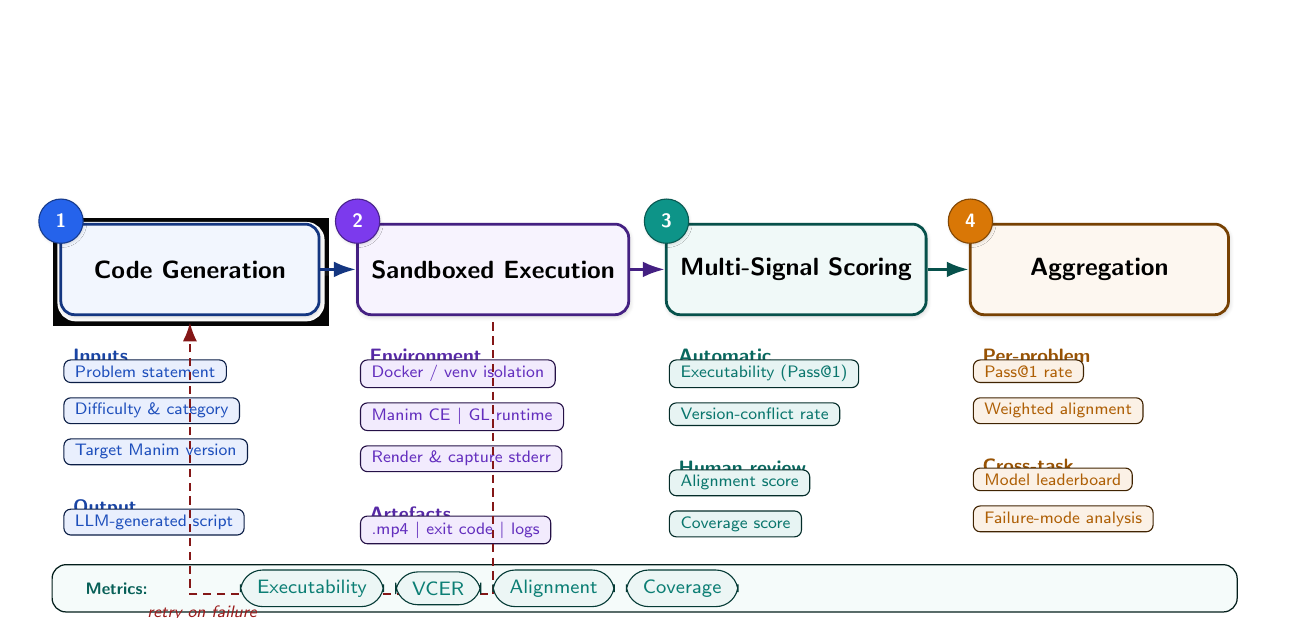
\begin{tikzpicture}[
        font=\sffamily\small,
        >=Latex,
    ]
        % ── Color palette ─────────────────────────────────────
        \definecolor{wfblue}{HTML}{2563EB}
        \definecolor{wfviolet}{HTML}{7C3AED}
        \definecolor{wfteal}{HTML}{0D9488}
        \definecolor{wforange}{HTML}{D97706}
        \definecolor{wfred}{HTML}{DC2626}
        \definecolor{panelbg}{HTML}{F8FAFC}
        \definecolor{panelborder}{HTML}{CBD5E1}
        \definecolor{trackgray}{HTML}{E2E8F0}

        % ── Shared styles ─────────────────────────────────────
        \tikzset{
            stage/.style 2 args={
                rectangle,
                rounded corners=5pt,
                draw=#1!55!black,
                line width=1pt,
                fill=#1!6,
                minimum width=3.28cm,
                minimum height=1.15cm,
                align=center,
                inner sep=5pt,
                blur shadow={shadow blur steps=6,
                             shadow xshift=0.4pt,
                             shadow yshift=-0.8pt,
                             shadow blur radius=1.6pt,
                             shadow opacity=18},
            },
            badge/.style 2 args={
                circle,
                draw=#1!60!black,
                fill=#1,
                text=white,
                inner sep=0pt,
                minimum size=16pt,
                font=\sffamily\scriptsize\bfseries,
                blur shadow={shadow blur steps=4,
                             shadow xshift=0.3pt,
                             shadow yshift=-0.5pt,
                             shadow blur radius=1pt,
                             shadow opacity=14},
            },
            bullet/.style 2 args={
                rectangle,
                rounded corners=2.5pt,
                draw=#1!30!black,
                fill=#1!10,
                inner xsep=4pt,
                inner ysep=2pt,
                font=\sffamily\fontsize{6.5}{8}\selectfont,
                text=#1!80!black,
            },
            metricpill/.style={
                rectangle,
                rounded corners=8pt,
                draw=wfteal!40!black,
                fill=wfteal!8,
                inner xsep=6pt,
                inner ysep=3.5pt,
                font=\sffamily\fontsize{6.8}{8.5}\selectfont,
                text=wfteal!85!black,
            },
            connector/.style={
                -{Latex[length=2.8mm, width=2mm]},
                line width=1.2pt,
                draw=#1!55!black,
            },
            feedbackarrow/.style={
                -{Latex[length=2.4mm, width=1.8mm]},
                line width=0.9pt,
                draw=wfred!60!black,
                densely dashed,
            },
            headerlabel/.style={
                font=\sffamily\fontsize{7.5}{9}\selectfont\bfseries,
                text=#1!70!black,
            },
        }

        % ── Coordinates ───────────────────────────────────────
        \coordinate (origin) at (0,0);
        \def\xsep{3.85}

        % ── Background panel ──────────────────────────────────
        \begin{scope}[on background layer]
            \fill[panelbg, rounded corners=8pt, draw=panelborder, line width=0.6pt]
                (-2.05, -4.55) rectangle ($(origin)+(\xsep*3+2.05, 2.55)$);
            % Title bar
            \fill[white, rounded corners=8pt]
                (-1.85, 1.95) rectangle ($(origin)+(\xsep*3+1.85, 2.38)$);
            \node[font=\sffamily\fontsize{7.8}{9}\selectfont\bfseries, text=black!60]
                at ($(origin)+(0.5*\xsep*3, 2.16)$)
                {\textsc{ManiBench} Evaluation Pipeline};
            % Horizontal track line
            \draw[trackgray, line width=2.8pt, line cap=round]
                (0, 0) -- +(\xsep*3, 0);
        \end{scope}

        % ══════════════════════════════════════════════════════
        % Stage 1 — Code Generation
        % ══════════════════════════════════════════════════════
        \node[stage={wfblue}{}] (gen) at (0,0)
            {\textbf{Code Generation}};

        \node[badge={wfblue}{}] at ($(gen.north west)+(0.02,0.02)$) {1};

        % Sub-items
        \node[headerlabel=wfblue, anchor=north west]
            at ($(gen.south west)+(0.05,-0.30)$) {Inputs};
        \node[bullet={wfblue}{}, anchor=north west] (g1)
            at ($(gen.south west)+(0.05,-0.55)$)
            {Problem statement};
        \node[bullet={wfblue}{}, anchor=north west] (g2)
            at ($(g1.south west)+(0,-0.18)$)
            {Difficulty \& category};
        \node[bullet={wfblue}{}, anchor=north west] (g3)
            at ($(g2.south west)+(0,-0.18)$)
            {Target Manim version};

        \node[headerlabel=wfblue, anchor=north west]
            at ($(g3.south west)+(0,-0.32)$) {Output};
        \node[bullet={wfblue}{}, anchor=north west] (g4)
            at ($(g3.south west)+(0,-0.55)$)
            {LLM-generated script};

        % ══════════════════════════════════════════════════════
        % Stage 2 — Sandboxed Execution
        % ══════════════════════════════════════════════════════
        \node[stage={wfviolet}{}] (exec) at (\xsep,0)
            {\textbf{Sandboxed Execution}};

        \node[badge={wfviolet}{}] at ($(exec.north west)+(0.02,0.02)$) {2};

        \node[headerlabel=wfviolet, anchor=north west]
            at ($(exec.south west)+(0.05,-0.30)$) {Environment};
        \node[bullet={wfviolet}{}, anchor=north west] (e1)
            at ($(exec.south west)+(0.05,-0.55)$)
            {Docker / venv isolation};
        \node[bullet={wfviolet}{}, anchor=north west] (e2)
            at ($(e1.south west)+(0,-0.18)$)
            {Manim CE \textbar{} GL runtime};
        \node[bullet={wfviolet}{}, anchor=north west] (e3)
            at ($(e2.south west)+(0,-0.18)$)
            {Render \& capture stderr};

        \node[headerlabel=wfviolet, anchor=north west]
            at ($(e3.south west)+(0,-0.32)$) {Artefacts};
        \node[bullet={wfviolet}{}, anchor=north west] (e4)
            at ($(e3.south west)+(0,-0.55)$)
            {.mp4 \textbar{} exit code \textbar{} logs};

        % ══════════════════════════════════════════════════════
        % Stage 3 — Multi-Signal Scoring
        % ══════════════════════════════════════════════════════
        \node[stage={wfteal}{}] (metric) at (2*\xsep,0)
            {\textbf{Multi-Signal Scoring}};

        \node[badge={wfteal}{}] at ($(metric.north west)+(0.02,0.02)$) {3};

        \node[headerlabel=wfteal, anchor=north west]
            at ($(metric.south west)+(0.05,-0.30)$) {Automatic};
        \node[bullet={wfteal}{}, anchor=north west] (s1)
            at ($(metric.south west)+(0.05,-0.55)$)
            {Executability (Pass@1)};
        \node[bullet={wfteal}{}, anchor=north west] (s2)
            at ($(s1.south west)+(0,-0.18)$)
            {Version-conflict rate};

        \node[headerlabel=wfteal, anchor=north west]
            at ($(s2.south west)+(0,-0.32)$) {Human review};
        \node[bullet={wfteal}{}, anchor=north west] (s3)
            at ($(s2.south west)+(0,-0.55)$)
            {Alignment score};
        \node[bullet={wfteal}{}, anchor=north west] (s4)
            at ($(s3.south west)+(0,-0.18)$)
            {Coverage score};

        % ══════════════════════════════════════════════════════
        % Stage 4 — Aggregation & Reporting
        % ══════════════════════════════════════════════════════
        \node[stage={wforange}{}] (agg) at (3*\xsep,0)
            {\textbf{Aggregation}};

        \node[badge={wforange}{}] at ($(agg.north west)+(0.02,0.02)$) {4};

        \node[headerlabel=wforange, anchor=north west]
            at ($(agg.south west)+(0.05,-0.30)$) {Per-problem};
        \node[bullet={wforange}{}, anchor=north west] (a1)
            at ($(agg.south west)+(0.05,-0.55)$)
            {Pass@1 rate};
        \node[bullet={wforange}{}, anchor=north west] (a2)
            at ($(a1.south west)+(0,-0.18)$)
            {Weighted alignment};

        \node[headerlabel=wforange, anchor=north west]
            at ($(a2.south west)+(0,-0.32)$) {Cross-task};
        \node[bullet={wforange}{}, anchor=north west] (a3)
            at ($(a2.south west)+(0,-0.55)$)
            {Model leaderboard};
        \node[bullet={wforange}{}, anchor=north west] (a4)
            at ($(a3.south west)+(0,-0.18)$)
            {Failure-mode analysis};

        % ══════════════════════════════════════════════════════
        % Connectors between stages (gradient-coloured)
        % ══════════════════════════════════════════════════════
        \draw[connector=wfblue]
            (gen.east) -- (exec.west);
        \draw[connector=wfviolet]
            (exec.east) -- (metric.west);
        \draw[connector=wfteal]
            (metric.east) -- (agg.west);

        % ── Feedback loop (retry on failure) ──────────────────
        \draw[feedbackarrow]
            ($(exec.south)+(0,-0.08)$)
            -- ++(0,-3.45)
            -| ($(gen.south)-(0,0.08)$)
            node[pos=0.48, below=0.5pt, font=\sffamily\fontsize{6}{7.5}\selectfont\itshape,
                 text=wfred!70!black] {retry on failure};

        % ══════════════════════════════════════════════════════
        % Metric pills — bottom banner
        % ══════════════════════════════════════════════════════
        \begin{scope}[on background layer]
            \fill[wfteal!4, rounded corners=5pt, draw=wfteal!20!black, line width=0.45pt]
                ($(origin)+(-1.75,-3.75)$)
                rectangle ($(origin)+(\xsep*3+1.75,-4.35)$);
        \end{scope}

        \node[font=\sffamily\fontsize{6.5}{8}\selectfont\bfseries, text=wfteal!65!black,
              anchor=west]
            at ($(origin)+(-1.45,-4.05)$) {Metrics:};

        \node[metricpill] (mp1) at ($(origin)+(1.55,-4.05)$)
            {Executability};
        \node[metricpill, right=4pt of mp1] (mp2)
            {VCER};
        \node[metricpill, right=4pt of mp2] (mp3)
            {Alignment};
        \node[metricpill, right=4pt of mp3] (mp4)
            {Coverage};

    \end{tikzpicture}
    \caption{The \textsc{ManiBench} evaluation pipeline.
    Each benchmark problem flows through four stages:
    \emph{(1)}~an LLM generates Manim code from a structured prompt;
    \emph{(2)}~the script executes inside a sandboxed, version-pinned environment;
    \emph{(3)}~automatic checks (executability, version-conflict rate) and human review
    (alignment, coverage) produce multi-signal scores; and
    \emph{(4)}~results are aggregated into per-problem and cross-task summaries.
    A dashed feedback loop indicates re-prompting on execution failure.}
    \label{fig:workflow}
\end{figure}

\subsection{Human Evaluation Protocol}
\label{sec:human-eval}

For Alignment and Coverage scores, we employ structured human evaluation:

\begin{enumerate}[nosep]
    \item Watch the rendered animation.
    \item Check off each required visual event as present or absent.
    \item Note timing: are events synchronized correctly?
    \item Assess pedagogical clarity: does the animation explain the concept?
    \item Provide Alignment Score ($0.0$--$1.0$) and Coverage Score ($0.0$--$1.0$).
\end{enumerate}

\noindent\textbf{Disagreement Resolution.}
Two independent reviewers score each output.
If disagreement exceeds~0.15, a third reviewer breaks the tie.
We report inter-rater agreement via Krippendorff's~$\alpha$ or Cohen's~$\kappa$.


\subsection{Automated Evaluation Framework}
\label{sec:auto-eval}

To complement human review and enable large-scale evaluation, we implement an automated evaluation pipeline.
The framework orchestrates code generation across multiple LLMs via the OpenRouter API, executes generated code in sandboxed environments, and computes all four metrics programmatically.

\subsubsection{Multi-Model Evaluation}

The pipeline supports six models spanning major LLM providers:

\begin{table}[ht]
    \centering
    \caption{Model roster for automated evaluation via OpenRouter.}
    \label{tab:models}
    \small
    \begin{tabular}{@{}lll@{}}
        \toprule
        \textbf{Model} & \textbf{Provider} & \textbf{OpenRouter ID} \\
        \midrule
        GPT-4o           & OpenAI    & \texttt{openai/gpt-4o-2024-11-20} \\
        Claude Sonnet~4  & Anthropic & \texttt{anthropic/claude-sonnet-4} \\
        Gemini 2.5~Pro   & Google    & \texttt{google/gemini-2.5-pro-preview} \\
        DeepSeek-R1      & DeepSeek  & \texttt{deepseek/deepseek-r1} \\
        Llama-4 Maverick & Meta      & \texttt{meta-llama/llama-4-maverick} \\
        Qwen-2.5 Coder   & Alibaba   & \texttt{qwen/qwen-2.5-coder-32b-instruct} \\
        \bottomrule
    \end{tabular}
\end{table}

All models are evaluated with temperature~$0.0$ for reproducibility, with a maximum of 8{,}192~generated tokens per request and 3~trials per (model, problem) pair.

\subsubsection{Automated Metric Computation}

Each generated code sample passes through a four-stage analysis pipeline:

\begin{enumerate}[nosep]
    \item \textbf{Syntax Validation:} Python AST parsing (\texttt{ast.parse}) to verify syntactic correctness.
    \item \textbf{Structural Checks:} detection of at least one \texttt{Scene} subclass and valid \texttt{from manim import *} imports; flagging of ManimGL-specific imports.
    \item \textbf{Sandboxed Execution:} the code is written to a temporary file and rendered via \texttt{subprocess} with a configurable timeout (default: 60\,s).
    Exit codes, \texttt{stderr}, and error types (\texttt{ImportError}, \texttt{AttributeError}, etc.) are captured.
    \item \textbf{Static Analysis:} over 40~regex patterns (derived from the 145~documented GL$\to$CE incompatibilities in Section~\ref{sec:refcode}) scan for version conflicts; keyword-bank--based heuristics detect the presence of required visual events and pedagogical elements.
\end{enumerate}

\noindent Executability and VCER are computed fully automatically.
Alignment and Coverage are approximated heuristically via keyword and AST matching, serving as lower-bound estimates pending human review.


\subsection{Prompt Engineering Strategies}
\label{sec:prompt-strategies}

Following the ManiBench Prompt Engineering Guide, we implement five prompting strategies of increasing sophistication:

\begin{enumerate}[nosep]
    \item \textbf{Zero-Shot Direct.}
    The problem statement is provided verbatim with a system prompt specifying Manim~CE as the target.
    Recommended for Level~1--2 problems; expected alignment: $0.80$--$0.90$.

    \item \textbf{Few-Shot Examples.}
    One or two working Manim~CE code examples precede the target problem.
    Examples are kept short (20--30~lines) and domain-relevant.
    Improves alignment by $+8$--$12\%$ and coverage by $+5$--$8\%$ over zero-shot.

    \item \textbf{Chain-of-Thought (CoT).}
    The model is instructed to first analyze visual components, event ordering, transformations, timing, and required labels before writing code.
    Improves alignment by $+10$--$15\%$ through better event ordering.

    \item \textbf{Constraint-Based.}
    Explicit timing, ordering, and criticality constraints are injected (e.g., ``gradient arrow must appear \emph{before} dot moves'').
    Most effective for Level~3--4 problems; improves alignment by $+15$--$20\%$.

    \item \textbf{Version-Conflict-Aware.}
    The system prompt enumerates forbidden ManimGL constructs (derived from Section~\ref{sec:refcode}), and problem-specific incompatibilities from the dataset's \texttt{version\_conflict\_notes} field are appended.
    Reduces version-conflict error rate from ${\sim}30\%$ to ${<}\,5\%$.
\end{enumerate}


%% ═══════════════════════════════════════════════════════════════
\section{Preliminary Results (Pilot Study)}
\label{sec:results}

\noindent\textbf{Setup:}
Models: GPT-4o, Claude~3.5 Sonnet (preliminary); full evaluation across all six models in Table~\ref{tab:models} is in progress.
Prompting: zero-shot (single problem prompt, no examples).
Manim version: CE\@.
Trials: 3~per model $\times$ 12~problems $= 72$~runs.

\begin{table}[ht]
    \centering
    \caption{Pilot study results across 12~benchmark problems.
    Executability is reported as the percentage of runs completing without error.
    Alignment and Coverage are averaged over successful runs; ``--'' indicates no successful execution.}
    \label{tab:results}
    \small
    \begin{tabular}{@{}lccccc@{}}
        \toprule
        \textbf{Problem} & \textbf{Diff.} & \textbf{Exec.\ (GPT-4o)} & \textbf{Exec.\ (Claude)} & \textbf{Avg Align.} & \textbf{Avg Cov.} \\
        \midrule
        1. Colliding Blocks  & 4 & 67\% & 67\% & 0.52 & 0.58 \\
        2. Gradient Descent   & 3 & 100\% & 100\% & 0.73 & 0.82 \\
        3. Convolution        & 3 & 0\%  & 33\% & --   & --   \\
        4. Eigenvectors       & 4 & 33\% & 33\% & 0.40 & 0.50 \\
        5. Determinant        & 2 & 100\% & 100\% & 0.85 & 0.88 \\
        6. CLT                & 3 & 0\%  & 33\% & --   & --   \\
        7. Medical Test       & 2 & 100\% & 100\% & 0.78 & 0.85 \\
        8. Chain Rule         & 3 & 67\% & 67\% & 0.60 & 0.68 \\
        9. Integration        & 3 & 0\%  & 33\% & --   & --   \\
        10. Taylor Series     & 4 & 33\% & 33\% & 0.35 & 0.42 \\
        11. Hairy Ball        & 5 & 0\%  & 0\%  & --   & --   \\
        12. Windmill          & 4 & 0\%  & 0\%  & --   & --   \\
        \bottomrule
    \end{tabular}
\end{table}

\noindent\textbf{Key Observations:}
\begin{enumerate}[nosep]
    \item \emph{Simple problems} (Determinant, Medical Test) achieve high executability (100\%) and alignment ($\ge 0.78$).
    \item \emph{Complex problems} (Convolution, CLT, Integration, Hairy Ball) show low executability (0--33\%), suggesting API misunderstandings or missing pedagogical elements.
    \item \emph{Drift events}: Problems requiring precise timing (Gradient Descent, Windmill) show lower alignment than coverage, indicating temporal synchronization issues.
    \item \emph{Version conflicts}: No GL-specific syntax was detected in this pilot; both models avoided GL references.
\end{enumerate}


%% ═══════════════════════════════════════════════════════════════
\section{Discussion}
\label{sec:discussion}

\subsection{Why ManiBench Matters}

Existing benchmarks (HumanEval, APPS) measure whether code produces correct \emph{output}.
\textsc{ManiBench} measures whether code produces correct \emph{understanding}.
This distinction is critical for educational tools, where a silent failure (wrong animation) is worse than a loud failure (runtime error).

\subsection{Limitations and Future Work}

\begin{enumerate}[nosep]
    \item \textbf{Alignment Scoring} is currently approximated via keyword-based heuristics in the automated pipeline, supplemented by manual review.
    Future work should explore automatic alignment detection via AST analysis, video-frame comparison, or vision--language model grading.
    \item \textbf{Pedagogical Validation.}
    We do not yet validate whether animations actually teach the concept.
    User studies with students could address this gap.
    \item \textbf{Manim API Coverage.}
    As Manim evolves, the benchmark should be versioned and updated accordingly.
    The 145~documented GL$\to$CE incompatibilities provide a starting point for automated version-conflict detection.
    \item \textbf{Scalability.}
    Moving from 12 to 150+ problems requires annotation infrastructure and community contribution.
    \item \textbf{Reference Code Utilization.}
    The ${\sim}53{,}000$~lines of analyzed reference code could enable fine-tuning studies or retrieval-augmented generation (RAG) experiments.
\end{enumerate}

\subsection{Broader Impact}

\textsc{ManiBench} can be used to:
\begin{itemize}[nosep]
    \item evaluate LLM educational-content generation,
    \item develop better prompting strategies for animation code,
    \item identify systematic failure modes (e.g., models struggling with temporal synchronization),
    \item drive research into improving Manim API adoption in LLMs,
    \item benchmark version-aware code generation using the 145~documented GL$\to$CE incompatibilities, and
    \item enable retrieval-augmented generation (RAG) experiments using the reference code analysis.
\end{itemize}


%% ═══════════════════════════════════════════════════════════════
\section{Conclusion}
\label{sec:conclusion}

We have introduced \textsc{ManiBench}, a specialized benchmark for evaluating Manim code generation.
By formalizing metrics for syntactic correctness, version compliance, visual-logic alignment, and pedagogical coverage, \textsc{ManiBench} moves beyond simple test-case evaluation to assess whether generated animations actually communicate mathematical concepts.

The 12-problem pilot dataset, backed by comprehensive reference code analysis of ${\sim}53{,}000$~lines of original 3Blue1Brown source code and 145~documented GL$\to$CE incompatibilities, demonstrates both the opportunities (simple concepts: ${\sim}80\%$ alignment) and challenges (complex temporal reasoning: ${\sim}40\%$ alignment) in automated animation generation.
The accompanying automated evaluation framework---supporting six LLMs across five prompting strategies---enables reproducible, large-scale assessment.
With planned expansion to 150--200 problems, \textsc{ManiBench} will serve as a foundational resource for advancing LLM-driven educational content creation.

The dataset and evaluation toolkit are publicly available at \url{https://huggingface.co/datasets/nabin2004/ManiBench}.


%% ═══════════════════════════════════════════════════════════════
\section*{References}
\label{sec:references}

\begin{enumerate}[nosep, label={[\arabic*]}]
    \item M.~Chen, J.~Tworek, H.~Jun, et al., ``Evaluating Large Language Models Trained on Code,'' \emph{arXiv:2107.03374}, 2021. (HumanEval)
    \item J.~Austin, A.~Odena, M.~Nye, et al., ``Program Synthesis with Large Language Models,'' \emph{arXiv:2108.07732}, 2021. (MBPP)
    \item D.~Hendrycks, S.~Basart, S.~Kadavath, et al., ``Measuring Coding Challenge Competence with APPS,'' \emph{NeurIPS Datasets and Benchmarks}, 2021.
    \item G.~Sanderson, ``3Blue1Brown,'' \url{https://www.3blue1brown.com/}, 2015--present.
    \item Manim Community Developers, ``Manim---Mathematical Animation Framework (Community Edition),'' \url{https://www.manim.community/}, 2020--present.
    \item G.~Sanderson, ``Manim (3Blue1Brown fork),'' \url{https://github.com/3b1b/manim}, 2015--present.
    \item T.~Brown, B.~Mann, N.~Ryder, et al., ``Language Models are Few-Shot Learners,'' \emph{NeurIPS}, 2020.
    \item J.~Wei, X.~Wang, D.~Schuurmans, et al., ``Chain-of-Thought Prompting Elicits Reasoning in Large Language Models,'' \emph{NeurIPS}, 2022.
    \item OpenAI, ``GPT-4o Technical Report,'' 2024.
    \item Anthropic, ``Claude Sonnet~4 Model Card,'' 2025.
    \item Google DeepMind, ``Gemini 2.5 Pro Technical Report,'' 2025.
    \item DeepSeek, ``DeepSeek-R1: Incentivizing Reasoning Capability in LLMs via Reinforcement Learning,'' \emph{arXiv:2501.12948}, 2025.
\end{enumerate}


%% ═══════════════════════════════════════════════════════════════
\appendix
\section{Problem Annotation Template}
\label{app:template}

Each problem in \textsc{ManiBench} is annotated as a JSON object with the following structured metadata:

\begin{description}[nosep]
    \item[\texttt{id}:] unique identifier (e.g., \texttt{MB-001}).
    \item[\texttt{title}:] descriptive title.
    \item[\texttt{youtube\_video\_id}:] YouTube video identifier.
    \item[\texttt{category}:] list of task categories (e.g., \texttt{["drift-sensitive", "multi-scene"]}).
    \item[\texttt{difficulty\_level}:] integer 1--5.
    \item[\texttt{domain}:] list of mathematical domain(s).
    \item[\texttt{full\_prompt}:] full natural-language problem statement (used as the LLM input).
    \item[\texttt{raw\_code\_status}:] whether original 3B1B source code has been collected.
    \item[\texttt{raw\_code\_path}:] relative path to original ManimGL source files.
    \item[\texttt{reference\_code\_analysis}:] structured analysis of original code, including:
    \begin{description}[nosep]
        \item[\texttt{framework}:] source framework (e.g., \texttt{manim\_gl}).
        \item[\texttt{total\_lines}:] lines of original code.
        \item[\texttt{scene\_classes}:] list of scene classes with descriptions and key methods.
        \item[\texttt{visual\_techniques}:] catalog of rendering and animation patterns.
        \item[\texttt{manim\_api\_patterns}:] updaters, animation types, 3D constructs, custom classes.
    \end{description}
    \item[\texttt{required\_visual\_events}:] list of events, each with an identifier, description, weight, criticality flag, timing, and reference code location.
    \item[\texttt{coverage\_requirements}:] list of required pedagogical elements.
    \item[\texttt{version\_conflict\_notes}:] GL$\to$CE incompatibilities specific to the problem.
    \item[\texttt{success\_criteria}:] minimum thresholds for executability, alignment, coverage, and version-conflict error rate.
    \item[\texttt{common\_failure\_modes}:] known LLM failure patterns with severity tags.
\end{description}

\noindent The full dataset is available in JSON format at \url{https://huggingface.co/datasets/nabin2004/ManiBench}.

\end{document}
